\documentclass[handout]{beamer}
%%%%%%%%%%%%%%%%%%%%%%%%%% DO NOT MODIFY %%%%%%%%%%%%%%%%%%%%%%%%%
%% preamble
\usetheme{Madrid}
\mode<presentation>
\usepackage[spanish]{babel}
\usepackage[utf8]{inputenc}
\usepackage{lmodern}
\usepackage{hyperref}
\usepackage{listings}
\usepackage[T1]{fontenc}

\defbeamertemplate*{footline}{shadow theme}{%
  \leavevmode%
  \hbox{\begin{beamercolorbox}[wd=.5\paperwidth,ht=2ex,dp=1ex,leftskip=.3cm plus1fil,rightskip=.3cm]{author in head/foot}%
      \usebeamerfont{author in head/foot}\hfill\insertshortauthor
  \end{beamercolorbox}%

  \begin{beamercolorbox}[wd=.5\paperwidth,ht=2ex,dp=1ex,leftskip=.3cm,rightskip=.3cm plus1fil]{title in head/foot}%
      \usebeamerfont{title in head/foot}\insertshorttitle\hfill%
  \insertframenumber\,/\,\inserttotalframenumber
  \end{beamercolorbox}}%
  \vskip0pt%
}

\AtBeginSection[]{
  \begin{frame}[allowframebreaks]{Contenido}
  \small{\tableofcontents[currentsection]}
  \end{frame}
}

\AtBeginSubsection[]{
  \begin{frame}[allowframebreaks]{Contenido}
    \small{\tableofcontents[currentsubsection]}
  \end{frame}
}
\beamertemplatenavigationsymbolsempty 
\usefonttheme[onlymath]{serif}

\lstdefinestyle{customHTML}{
  belowcaptionskip=1\baselineskip,
  breaklines=true,
  frame=L,
  xleftmargin=\parindent,
  language=HTML,
  showstringspaces=false,
  basicstyle=\footnotesize\ttfamily,
  keywordstyle=\bfseries\color{blue},
  commentstyle=\itshape\color{gray},
  identifierstyle=\color{black},
  stringstyle=\color{orange},
}
\lstset{escapechar=@,style=customHTML}

%%%%%%%%%%%%%%%%%%%%%%%%% END DO NOT MODIFY %%%%%%%%%%%%%%%%%%%%

\title{Introducción a la Programación}
\subtitle{Variables}
\author{Edwin Salvador}
\date{21 de junio de 2016}
\begin{document}
  \begin{frame}
    \titlepage
    \centerline{Clase 10}
  \end{frame}
  
  \AtBeginSection[]{
    \begin{frame}[allowframebreaks]{Contenido}
      \tableofcontents[currentsection]
    \end{frame}
  }

\section{El operador \% (``módulo'' o ``resto'')} % (fold)
\label{sec:el_operador__modulo_o_resto_}
\begin{frame}[t]\frametitle{El operador \% (``módulo'' o ``resto'')}
    
\texttt{int a = 5;}\\
\texttt{int b = 3;} \\
\texttt{int r = a \% b;}


\end{frame}

\begin{frame}[t]\frametitle{Ejemplo módulo}
    \begin{itemize}
      \item Verificar si el número que ingresa el usuario por teclado es par o impar       
    \end{itemize}

    \begin{figure}[tb]
      \centering
      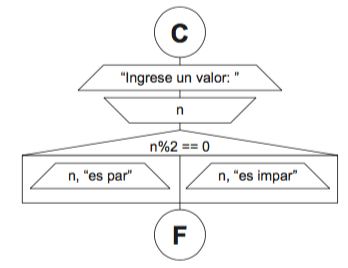
\includegraphics[scale=.7]{./img/mod}
    \end{figure}

\end{frame}
% section el_operador__modulo_o_resto_ (end)

\section{Operadores Relacionales} % (fold)
\label{sec:operadores_relacionales}
\begin{frame}[t]\frametitle{Operadores Relacionales}
    
\begin{figure}[tb]
  \centering
  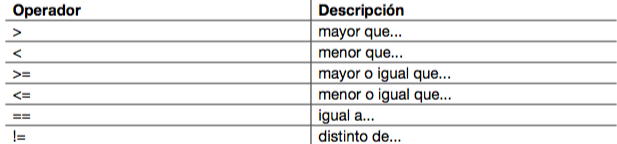
\includegraphics[scale=.6]{./img/oprela}
\end{figure}

\end{frame}
% section operadores_relacionales (end)

\section{Expresiones lógicas} % (fold)
\label{sec:exmpresiones_logicas}
\begin{frame}[t]\frametitle{Expresiones lógicas}
        
\begin{itemize}
  \item Pueden ser verdaderas o falsas
  \item 2 < 5
  \item 2 + 1 = 4
  \item Hola = Hola
\end{itemize}
\end{frame}

\begin{frame}[t]\frametitle{Operadores lógicos}
    
\begin{figure}[tb]
  \centering
  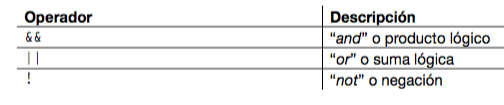
\includegraphics[scale=.7]{./img/oplog}
\end{figure}

\end{frame}

\begin{frame}[t]\frametitle{Operadores AND (\&\&)}
    
\begin{figure}[tb]
  \centering
  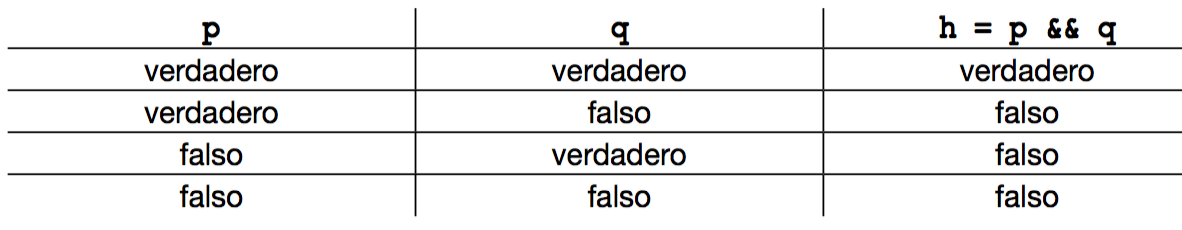
\includegraphics[scale=.5]{./img/oplog1}
\end{figure}

\end{frame}

\begin{frame}[t]\frametitle{Operadores OR (||)}
    
\begin{figure}[tb]
  \centering
  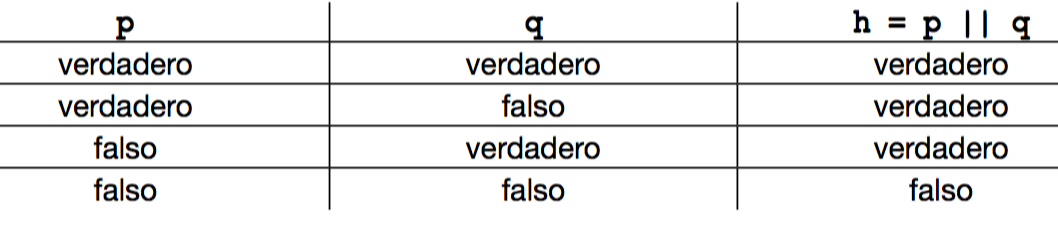
\includegraphics[scale=.5]{./img/oplogOR}
\end{figure}

\end{frame}

\begin{frame}[t]\frametitle{Operadores NOT (!)}
    
\begin{figure}[tb]
  \centering
  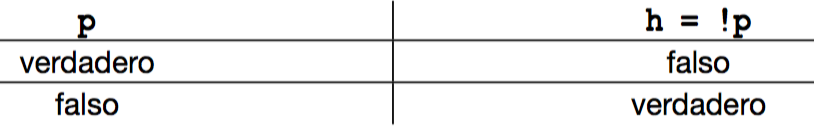
\includegraphics[scale=.5]{./img/oplogNOT}
\end{figure}

\end{frame}
% section expresiones_lógicas (end)

\section{Estructuras de control} % (fold)
\label{sec:estructuras_de_control}
\subsection{Estructura de Decisión} % (fold)
\label{sub:estructura_de_decision}

\begin{frame}[t]\frametitle{Estructura de decisión}
    
Ejemplo
\begin{itemize}
  \item Leer dos valores numéricos enteros e indicar cuál es el mayor y cuál es el menor. Considerar que ambos valores son diferentes.
  \begin{figure}[tb]
     \centering
     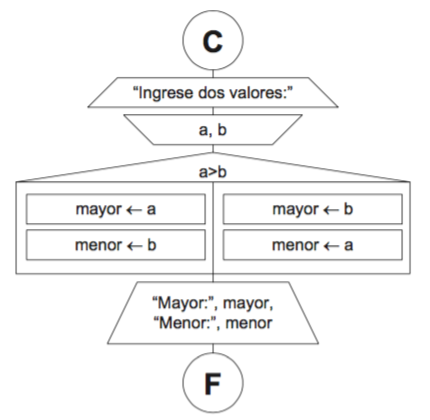
\includegraphics[scale=.7]{./img/if}
   \end{figure} 
\end{itemize}


\end{frame}

\begin{frame}[t]\frametitle{Estructuras de decisión anidadas}
    
Cuando una estructura de decisión está dentro de otra. Ejemplo:
\begin{itemize}
  \item Leer tres valores numéricos enteros, indicar cuál es el mayor, cuál es el del medio y cuál, el menor. Considerar que los tres valores serán diferentes.
  \begin{figure}[tb]
    \centering
    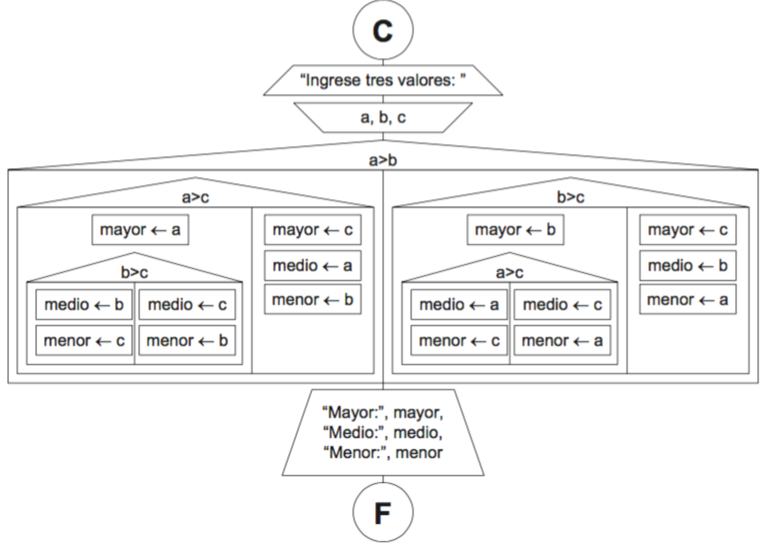
\includegraphics[scale=.6]{./img/ifani}
  \end{figure}
 
\end{itemize}


\end{frame}

\begin{frame}[t]\frametitle{Una mejor solución al ejercicio anterior}
    Es mejor evitar anidar muchos \texttt{if}, para eso podemos utilizar los operadores lógicos y también el \textbf{if en una línea}
\begin{figure}[tb]
  \centering
  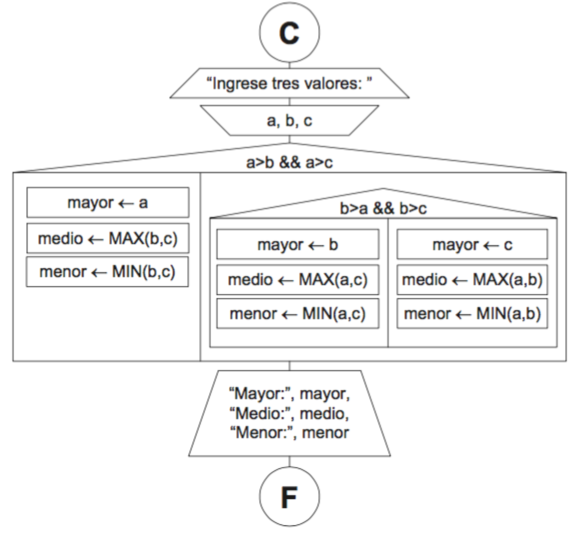
\includegraphics[scale=.6]{./img/ifani2}
\end{figure}

\end{frame}

\begin{frame}[t]\frametitle{Selección múltiple (\texttt{switch})}
    
\begin{figure}[tb]
    \centering
    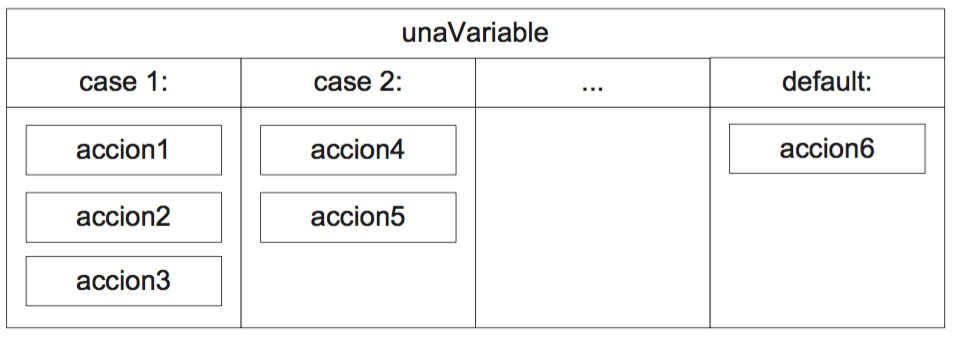
\includegraphics[scale=.7]{./img/explicacionswitch}
\end{figure}

\end{frame}

\begin{frame}[t,fragile]\frametitle{Estructura del \texttt{switch}}
    
\begin{lstlisting}
switch(expresion) {
    case expresion_cte_1:
        sentencia_1;
    break;
    case expresion_cte_2:
        sentencia_2;
    break;
    .
    .
    .
    case expresion_cte_n:
        sentencia_n; 
    break;
    [default: 
        sentencia;]
}
\end{lstlisting}
\end{frame}

\begin{frame}[t,fragile]\frametitle{\texttt{strcpy}}
    
\begin{lstlisting}
// defino un "conjunto" de 10 variables de tipo char
char s[10];
// strcpy asigna cada uno de los caracteres de "Hola" // a cada una de las variables del conjunto s 
strcpy(s,"Hola"); 
\end{lstlisting}
\begin{figure}[tb]
    \centering
    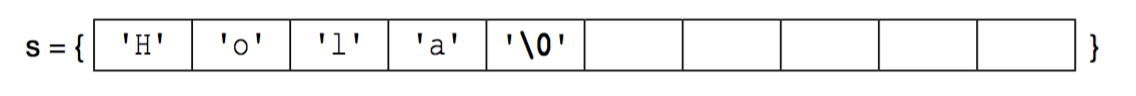
\includegraphics[scale=.6]{./img/strcpy}
\end{figure}

\texttt{strcpy} agrega el caracter especial \texttt{\textbackslash{0}} (barra cero) que delimita el final de la cadena.\\
Para la cadena \texttt{Hola}, se necesitan 5 caracteres \texttt{Hola} más el \texttt{\textbackslash{0}}\\
Se puede asignar el valor de la cadena con el sigo \texttt{=} solo cuando se define la variable.
\begin{lstlisting}
char nombre[] = "Pablo"; 
\end{lstlisting}
\end{frame}

\begin{frame}[t]\frametitle{Ejemplo \texttt{switch}}
    
Leer un valor numérico que representa un día de la semana. Se pide mostrar por pantalla el nombre del día considerando que el lunes es el día 1, el martes es el día 2 y así, sucesivamente.

\begin{figure}[tb]
    \centering
    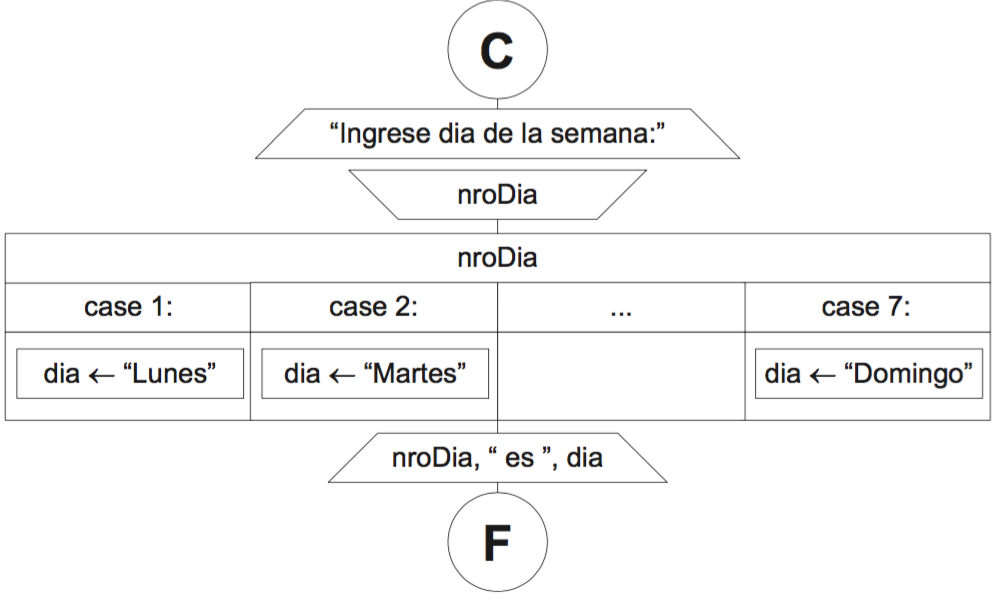
\includegraphics[scale=.6]{./img/ejswitch}
\end{figure}

\end{frame}


% subsection estructura_de_decisión (end)
% section estructuras_de_control (end)
\end{document}
